\documentclass[10pt,a4paper,twoside]{article}
% The following LaTeX packages must be installed on your machine: amsmath, authblk, bm, booktabs, caption, dcolumn, fancyhdr, geometry, graphicx, hyperref, latexsym, natbib

% Please make sure that spp.dat (supplied with this template) is in your working directory or path
\usepackage{physics}
\usepackage{amssymb}
\usepackage{subcaption}
\input{spp.dat}

%  Editorial staff will uncomment the next line
 \providecommand{\artnum}[0]{PB-38}
 \renewcommand{\articlenum}[0]{SPP-2019-PB-38-}

\begin{document}

%--------------------------------------------------
%  Fill in the paper's title in Sentence case
%  Titles beginning with articles (A, An, The) are discouraged
%--------------------------------------------------
\title{\TitleFont Frequency domain reconstruction of stochastically sampled signals based on compressive sensing}


%--------------------------------------------------
% For TWO authors with the same affiliation please use this block
% Or Please use the other author block templates
%--------------------------------------------------
\author[*\negthickspace]{Kenneth V. Domingo}
\author[ ]{Maricor N.~Soriano
\lastauthorsep}
\affil[ ]{National Institute of Physics, University of the Philippines Diliman}
\affil[*]{\corremail{kdomingo@nip.upd.edu.ph} }

%--------------------------------------------------
%  For three or more authors with the same affiliation please use this block
%--------------------------------------------------

% \author[*]{Author M.~Surname\authorsep}
% \author[ ]{Bauthor D.~Surname~Jr.\authorsep}
% \author[ ]{Cauthor D.~Surname~III\lastauthorsep}
% \affil[ ]{Department of Science, XXX University, Country}
% \affil[*]{\corremail{amsurname@university.edu} }

%--------------------------------------------------
%  For authors with different affiliations please use the following block
%--------------------------------------------------
% \author[1*]{Author M.~Surname\authorsep}
% \author[2]{Bauthor D.~Surname~Jr.\authorsep}
% \author[1,2]{Coauthor G.~Surname~III\authorsep}
% % !!! Please take note that the last author separation is \lastauthorsep instead of \authorsep
% \author[3]{Dauthor G.~Surname\lastauthorsep}
% \affil[1]{Department of Physics, DD University, Country}
% \affil[2]{Department of Science, XX University, Country}
% \affil[3]{Physics Institute, Country}
% \affil[*]{\corremail{amsurname@university.edu} }


\begin{abstract}
\noindent
%--------------------------------------------------
% Include abstract and keywords here
%--------------------------------------------------
The field of compressed sensing (CS) has recently been gaining traction as a viable workaround to the Nyquist-Shannon sampling theorem (NSST). This allows highly accurate signal recovery from incomplete frequency information. In this paper, we investigate the ability of compressive sampling to recover the higher harmonics of a recorded guitar signal. Sampling is done in the temporal domain, and the reconstruction is performed in the frequency domain. It is shown that even when taking a small number of random samples corresponding to some underlying sub-Nyquist rate, the base frequency, including up to fifth-order harmonics, can be recovered. The performance of three algorithms, namely least absolute shrinkage and selection operator (LASSO), orthogonal matching pursuit (OMP), and smoothed $\ell^0$ norm (SL0) algorithm in terms of computation time and reconstruction error (cosine similarity) were investigated.

\keywords{compressive sensing, norm minimization, signal processing.}

\end{abstract}

\maketitle
\thispagestyle{titlestyle}


%--------------------------------------------------
% the main text of your paper begins here
%--------------------------------------------------
\section{Introduction}\label{sec:intro}
The Nyquist-Shannon sampling theorem (NSST), in the field of analog-to-digital conversion, states that in order to digitally reconstruct a real signal, whose highest frequency component is indicated as $f_B$, and without losing any of the information contained in it, an analog-to-digital converter (ADC) must sample it at a rate $f_S$ that is at least twice this frequency; that is,

\begin{equation}\label{eq:nyquistshannon}
	f_S \geq 2f_B
\end{equation}

where the sampling rate $f_S$, if \eqref{eq:nyquistshannon} were to be treated as an equality, is known as the Nyquist rate. However, signal transmissions that utilize frequencies higher up the electromagnetic spectrum cause a need for shorter sampling periods, and maintaining precise periodic sampling on the order of nanoseconds becomes impractical to implement on ADC hardware. The emerging field of compressed sensing (CS) introduced by Cand\`{e}s, Romberg, Tao \cite{candes}, and Donoho \cite{donoho} treats the entire process of signal acquisition, conversion, and reconstruction as an underdetermined linear system, which allows sampling signals at a rate much lower than that required by the NSST. Such a linear system, subject to specific constraints, can be solved using various methods implemented on hardware and/or software.

Mathew and Premanand \cite{mathew} proposed a compressive sensing method that uses a measurement matrix built from a chaotic logistic map to ensure incoherence between itself and the orthonormalization matrix. Andr\'{a}\v{s}, Dolinsk\'{y}, and \v{S}aliga \cite{andras} perform reconstruction of undersampled, one-dimensional, temporal signals directly in the time domain using stochastic sampling, as opposed to periodic, sub-Nyquist sampling. Romero, Tapang, and Saloma \cite{romero16,romero18} perform compressive sampling of 2D signals (images) directly in the Fourier domain and reconstruct via total variation minimization.

In this paper, we compare the performance of compressive sensing algorithms in reconstructing temporal signals in terms of speed and signal quality. We apply these to recorded acoustic signals by stochastically sampling directly in the temporal domain, and performing reconstruction in the frequency domain using weighted regularization, greedy, or convex optimization algorithms. Similar to Mathew, we perform compressive sampling on pure sinusoidal tones, and examine running time of different recovery algorithms. In contrast with Romero, we perform compressive sampling of 1D signals in the temporal domain, and reconstruct in the frequency domain via norm minimization. We tackle this research with the eventual goal of determining the frequency characteristics of compressively sampled signals for applications such as speech recording.

\section{Methodology}\label{sec:Metho}
\medskip

\subsection{Compressive sensing}\label{ssec:CS}
Consider a real-valued, one-dimensional signal $\vec{x}$, with length $N$. Let $\bm\Psi$ be some $N \times N$ sparse orthonormal basis whose column vectors can be represented as $\psi_i$. It is assumed that the signal $\vec{x}$ can be fully represented by a linear combination of $\psi_i$'s, or

\begin{equation}\label{eq:sparserep}
	\vec{x} = \bm\Psi\bm\alpha = \sum_i^N \alpha_i \psi_i
\end{equation}

where $\alpha_i$ are the sparse domain coefficients. A signal $\vec{x}$ is said to be $k$-sparse in the $\bm\Psi$ domain if it has, at most, $k$ non-zero coefficients. The compressed signal $\vec{y}$ of length $M$ ($M \ll N$) is

\begin{equation}\label{eq:compressedsig}
	\vec{y} = \bm\Phi\vec{x}
\end{equation}

where $\bm\Phi$ is referred to as the measurement matrix or sensing matrix. In order to successfully reconstruct $\vec{x}$ from $\vec{y}$, the sensing matrix must obey the restricted isometry property and be incoherent with the orthonormalization matrix $\bm\Psi$ so that sparsity is maintained. The goal for CS recovery algorithms then is to search for the sparsest signal $\vec{x}$ that yields $\vec{y}$, formalized as

\begin{equation}\label{eq:minimize}
	\min \norm{\vec{x}}_0 \quad \textrm{subject to} \quad \bm\Phi\vec{x} = \vec{y}
\end{equation}

where the notation $\norm{\vec{x}}_p$ denotes the $\ell_p$-norm of a vector $\vec{x}$. The $\ell_0$ pseudo-norm returns the number of non-zero elements in $\vec{x}$. Computational complexity can be reduced by applying certain constraints and minimizing the $\ell_1$-norm instead, defined as

\begin{equation}\label{eq:l1norm}
	\norm{\vec{x}}_1 = \sum_i \abs{x_i}
\end{equation}

\subsection{Stochastic sampling}\label{ssec:subsample}
The acoustic signal $\vec{x}$ with length $N$ is sampled at $M$ uniformly distributed random points in the signal. This is done so that there is no coherent aliasing effect, as opposed to sub-Nyquist periodic sampling, which loses all information regarding frequencies beyond the Nyquist rate. The number of random samples is chosen while taking into account the underlying Nyquist rate, i.e. if the Nyquist rate is $f_B$ Hz, we take $< f_B$ random samples. The sampling process can be visualized as

\begin{equation}\label{eq:randomsample}
	\vec{y} = \sum_{r_i} x_{r_i}, \quad r_i \in \textrm{random}\left[ 0, N \right) \in \mathbb{Z}
\end{equation}

A guitar playing a single note was used as a test signal to demonstrate compressive sensing on a temporal signal. The audio signals were first sampled at the standard 44.1 kHz. Since the sensing matrix scales with the input signal accordingly with a factor $MN$, it is impractical to process the entire signal at that rate for more than $1/8$ of a second. Thus, we downsample the input signal to a rate such that the desired $n$th-order harmonic is preserved, i.e. we satisfy the NSST for the harmonic frequency of our choosing. We then take $M$ uniformly distributed random samples from this downsampled signal and feed it into the preferred reconstruction algorithm.

\subsection{Construction of orthonormal and measurement bases}\label{ssec:bases}
The orthonormal basis $\bm\Psi$, in the context of CS, is generally chosen such that it is easy to generate and yields a real-valued output, thereby reducing computation time; in this case, a discrete cosine transform (DCT) matrix. The measurement basis $\bm\Phi$ is composed of randomly selected rows of $\bm\Psi$. The indices corresponding to the obtained random data points in Sec. \ref{ssec:subsample} are the same indices corresponding to the rows of $\bm\Psi$ that are to be taken. To wit,

\begin{equation}\label{eq:constructbasis}
	\bm\Phi = \mqty[ \qty(\psi^\top)_{r_1} & \qty(\psi^\top)_{r_2} & \hdots  & \qty(\psi^\top)_{r_M} ]^\top
\end{equation}

where $\qty(\psi^\top)_{r_i}$ are the $r_i$th row vectors of $\bm\Psi$.

\subsection{Signal reconstruction methods}\label{ssec:recon}
Many algorithms exist that attempt to solve underdetermined linear systems using a variety of approaches. The ones which are utilized here involve least absolute shrinkage and selection operator (LASSO) \cite{pyrunner}, which has the optimization objective

\begin{equation}\label{eq:lasso}
	\frac{1}{2M} \norm{\vec{y} - \bm\Phi w}_2^2 + \alpha \norm{w}_1
\end{equation}

where $w$ is some loss function and $\alpha$ is a regularization parameter; orthogonal matching pursuit (OMP) \cite{sklearn}, which has the approximation objective

\begin{equation}\label{eq:omp}
	\min_x \norm{\vec{y} - \bm\Phi\vec{x}}_2^2 \quad \textrm{subject to} \quad \norm{\vec{x}}_0 \leq M
\end{equation}

and smoothed $\ell^0$ norm (SL0) algorithm \cite{sl0} which attempts to approximate the $\ell_0$-norm directly using a Gaussian function of the form

\begin{equation}\label{eq:sl0-kernel}
	\lim_{\sigma \rightarrow 0} x_i \exp(-\frac{x_i^2}{2\sigma^2})
\end{equation}

\subsection{Performance evaluation}
\label{ssec:eval}
Reconstruction error was evaluated using the cosine similarity

\begin{equation}\label{eq:cossim}
	\textrm{similarity} = \cos{\theta} = \frac{\vec{x} \cdot \hat{\vec{x}}}{\norm{\vec{x}}_2 \norm{\hat{\vec{x}}}_2}
\end{equation}

where $\vec{x}$ and $\hat{\vec{x}}$ are the normalized original and reconstructed signals, respectively.

\section{Results and Discussion}\label{sec:RnD}

To investigate the CS algorithm's performance with real acoustic signals while factoring in noise, an acoustic guitar playing a single E$_4$ (330 Hz) note sampled at 8 kHz for 4 seconds was recorded. Figure \ref{fig:record-orig} shows the frequency domain representation with an inset time domain representation. The frequency spectrum evidently shows the base frequency as the highest peak and its harmonics as the succeeding peaks. Compressive sampling was performed directly in the temporal domain, and a sampling rate of 1 kHz was selected, corresponding to 4000 samples or 50\% of the original number of samples, which also corresponds to satisfying the Nyquist criterion for frequencies $\leq$ 500 Hz. The compressed signal's frequency domain representation with an inset temporal domain representation is shown in Fig. \ref{fig:record-comp}, and it can be observed that information is smeared throughout the entire frequency spectrum. Reconstruction was performed using LASSO, and the result is shown in Fig. \ref{fig:record-recon-lasso}. The frequency domain representation shows successful recovery of the base frequency, along with the first five harmonics, which are easily distinguishable from the noise. In the temporal domain representation, the amplitude envelope also closely mirrors the original, with the exception of additional audible noise at the release stage of the envelope.

Table \ref{tab:compare} compares the performances of the three algorithms in terms of running time and reconstruction error. In terms of running time, OMP converges fastest for a few samples, but runtime scales quadratically as the number of samples is increased. LASSO and SL0 scale almost linearly. Above 30\% of samples, SL0 performs fastest, closely followed by LASSO, then OMP. In terms of cosine similarity, however, LASSO consistently produces the least error, followed by SL0, with OMP performing poorly with a large deviation. Figures \ref{fig:process-time}-\ref{fig:cossim} show how the runtime and similarity scale with the number of samples to be processed.

\begin{table}[!htb]
	\centering
	\caption{Runtime and cosine similarity per algorithm using 50\% of original samples, average over 10 iterations.}
	\begin{tabular}{|c|c|c|c|}
		\hline
		Algorithm & Runtime & Cosine similarity \\ \hline
		LASSO & 49 s & $0.888 \pm 0.003$ \\
		OMP & 180 s & $0.351 \pm 0.209$ \\ 
		SL0 & 74 s & $0.823 \pm 0.020$ \\ \hline
	\end{tabular}
	\label{tab:compare}
\end{table}

\begin{figure}[!htb]
	\centering
	\begin{subfigure}{0.32\linewidth}
		\centering
		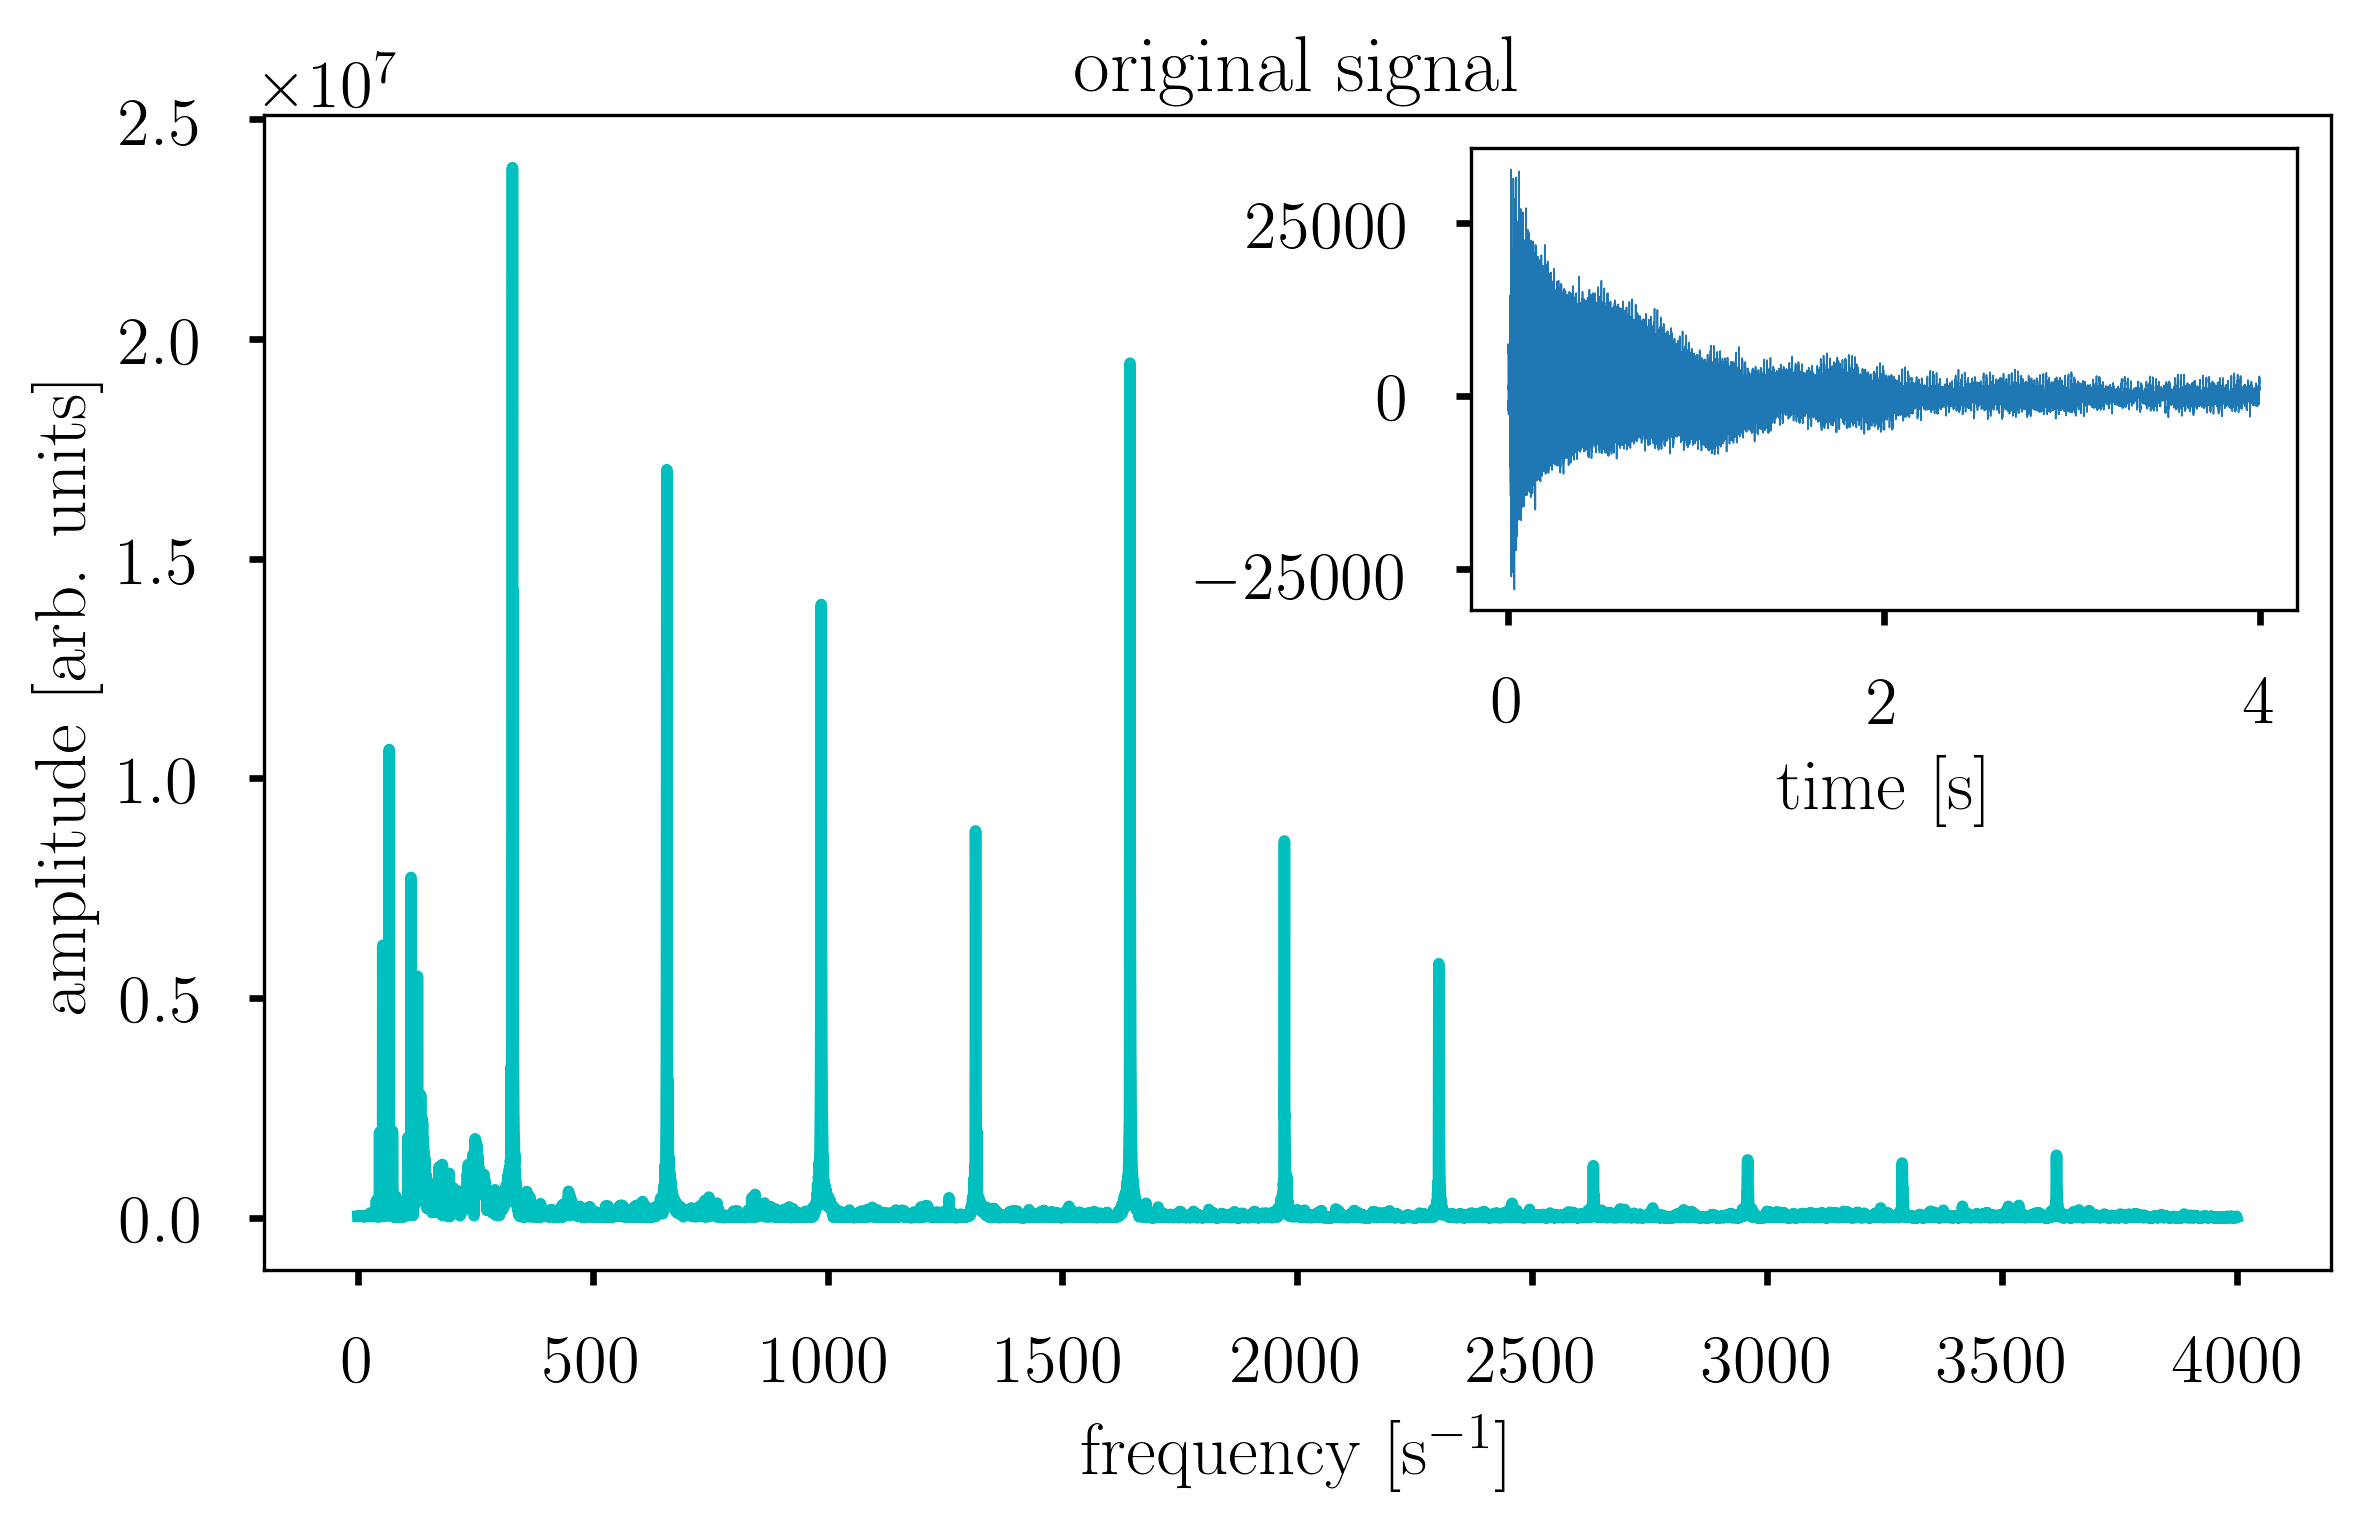
\includegraphics[width=\linewidth]{E1_original.png}
		\caption{original signal}
		\label{fig:record-orig}
	\end{subfigure}
	\begin{subfigure}{0.32\linewidth}
		\centering
		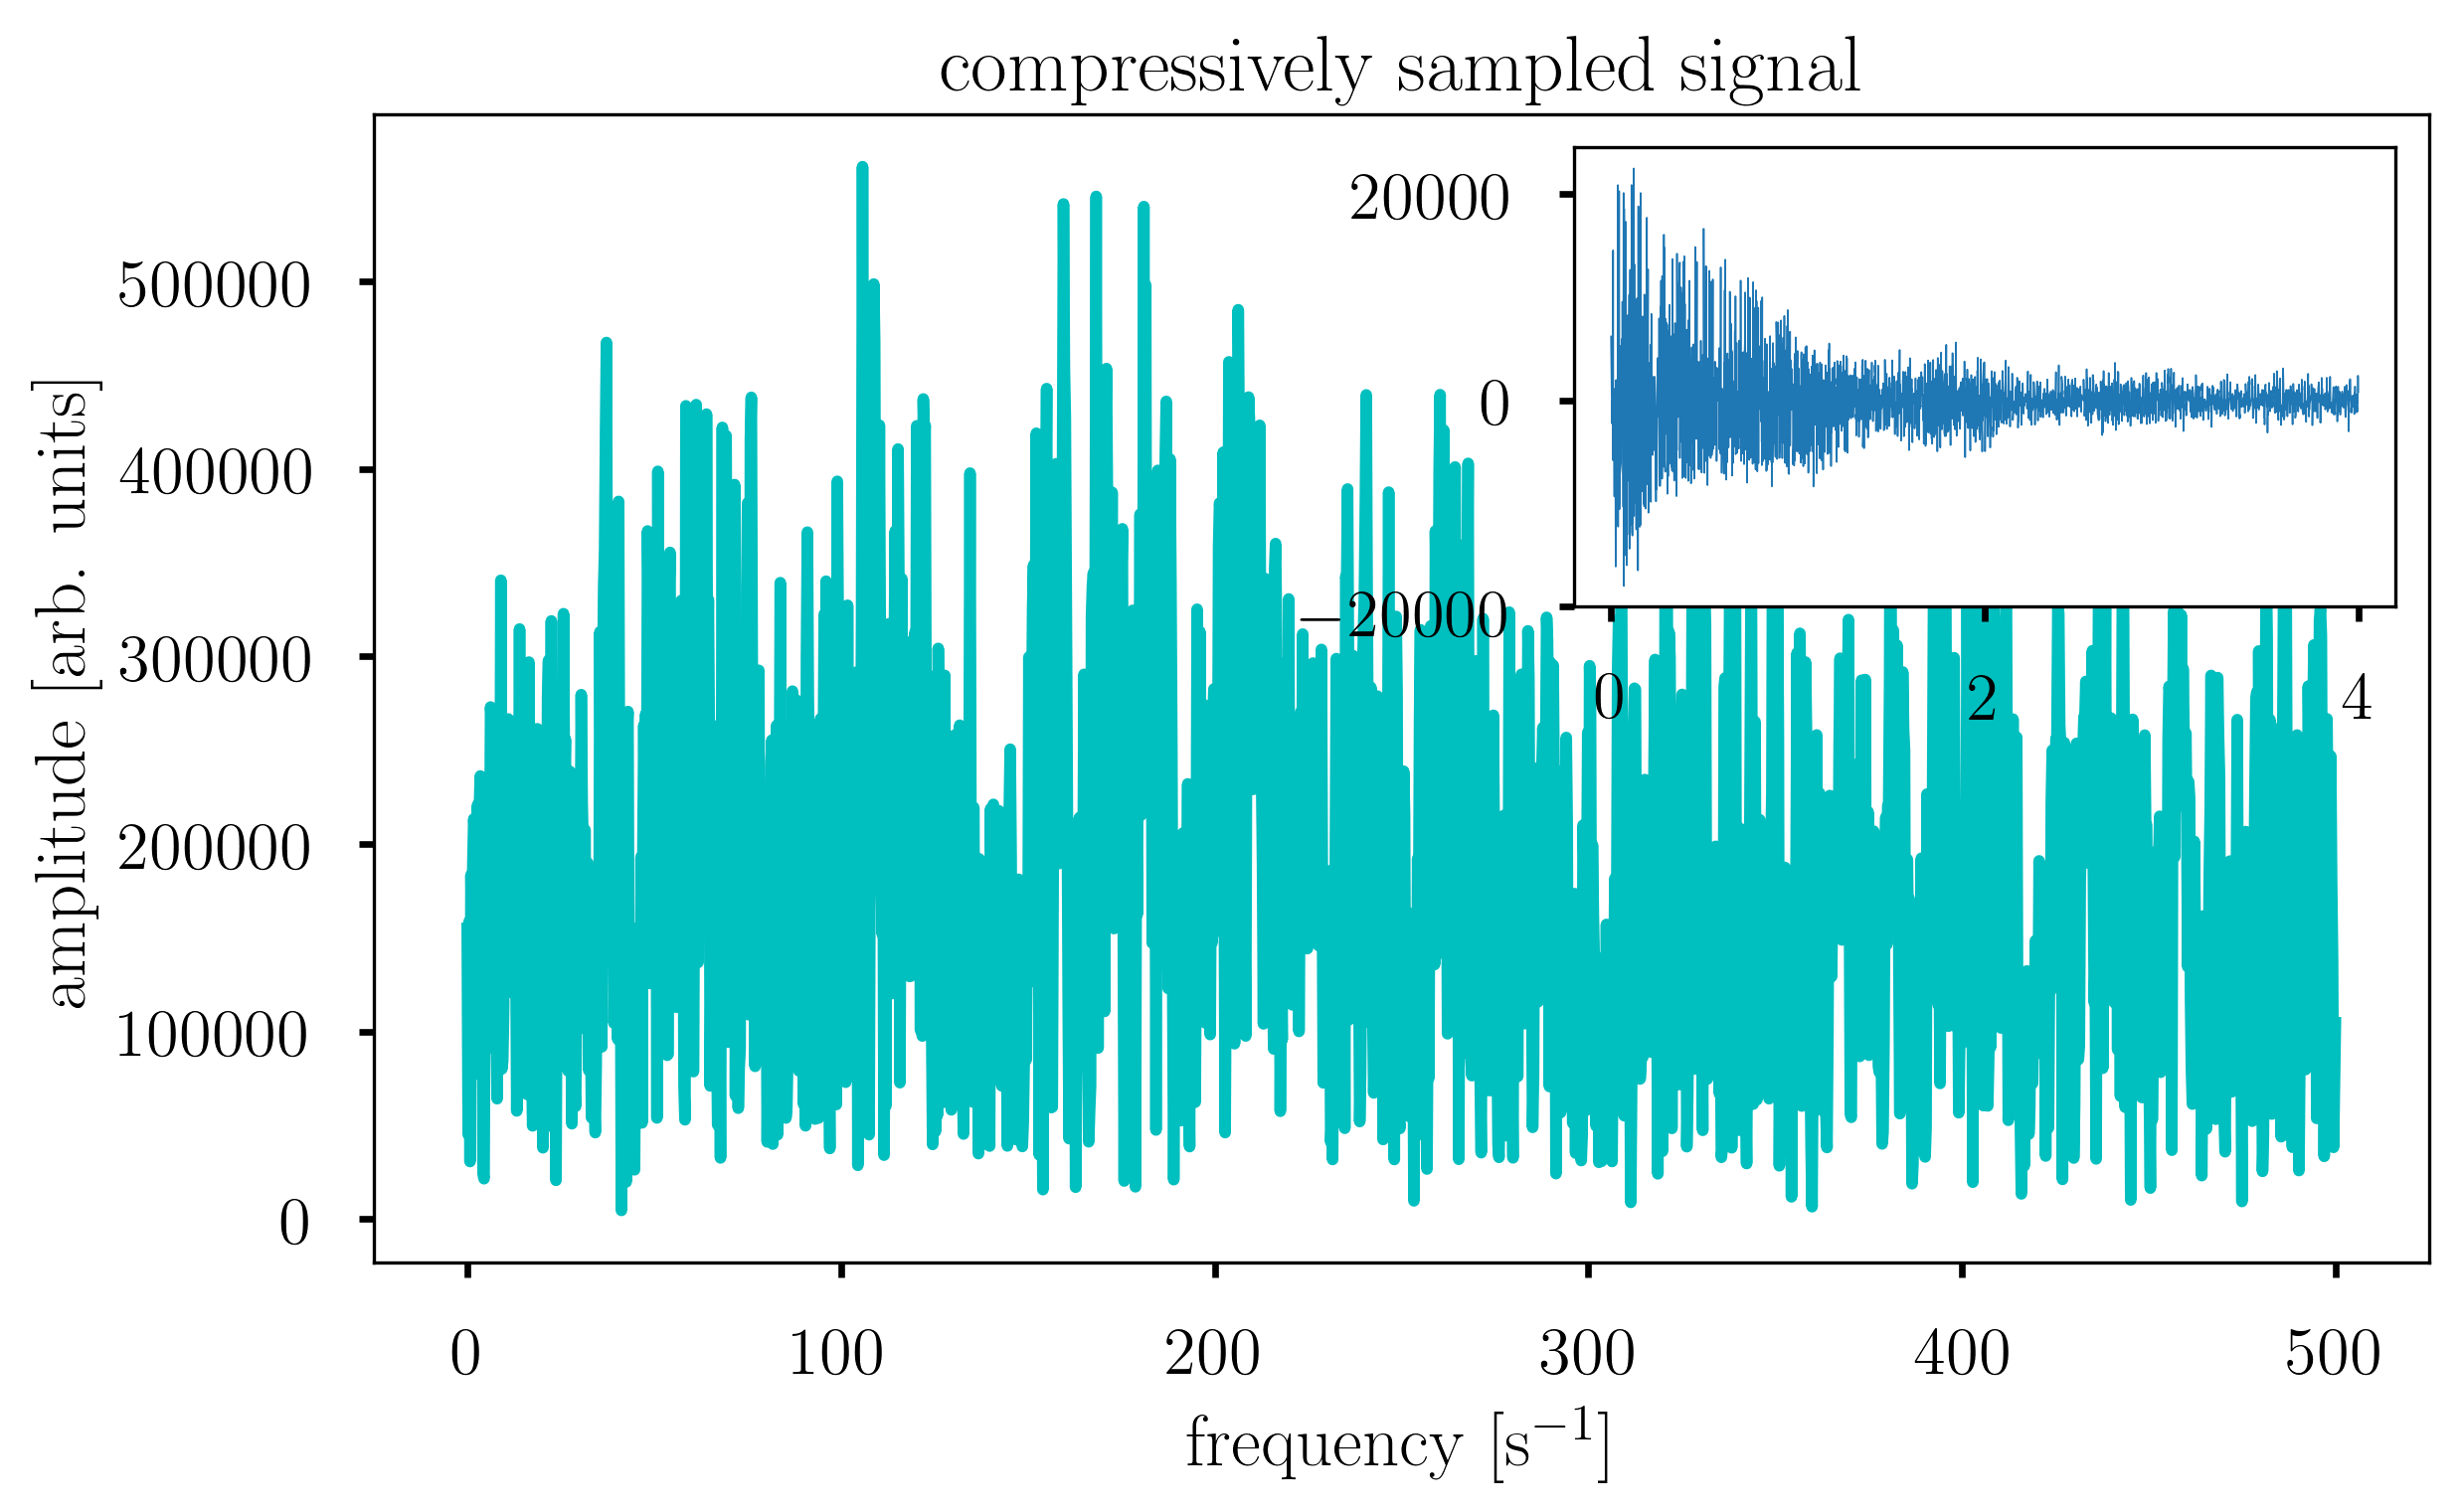
\includegraphics[width=\linewidth]{E1_comp.png}
		\caption{compressively sampled signal}
		\label{fig:record-comp}
	\end{subfigure}
	\begin{subfigure}{0.32\linewidth}
		\centering
		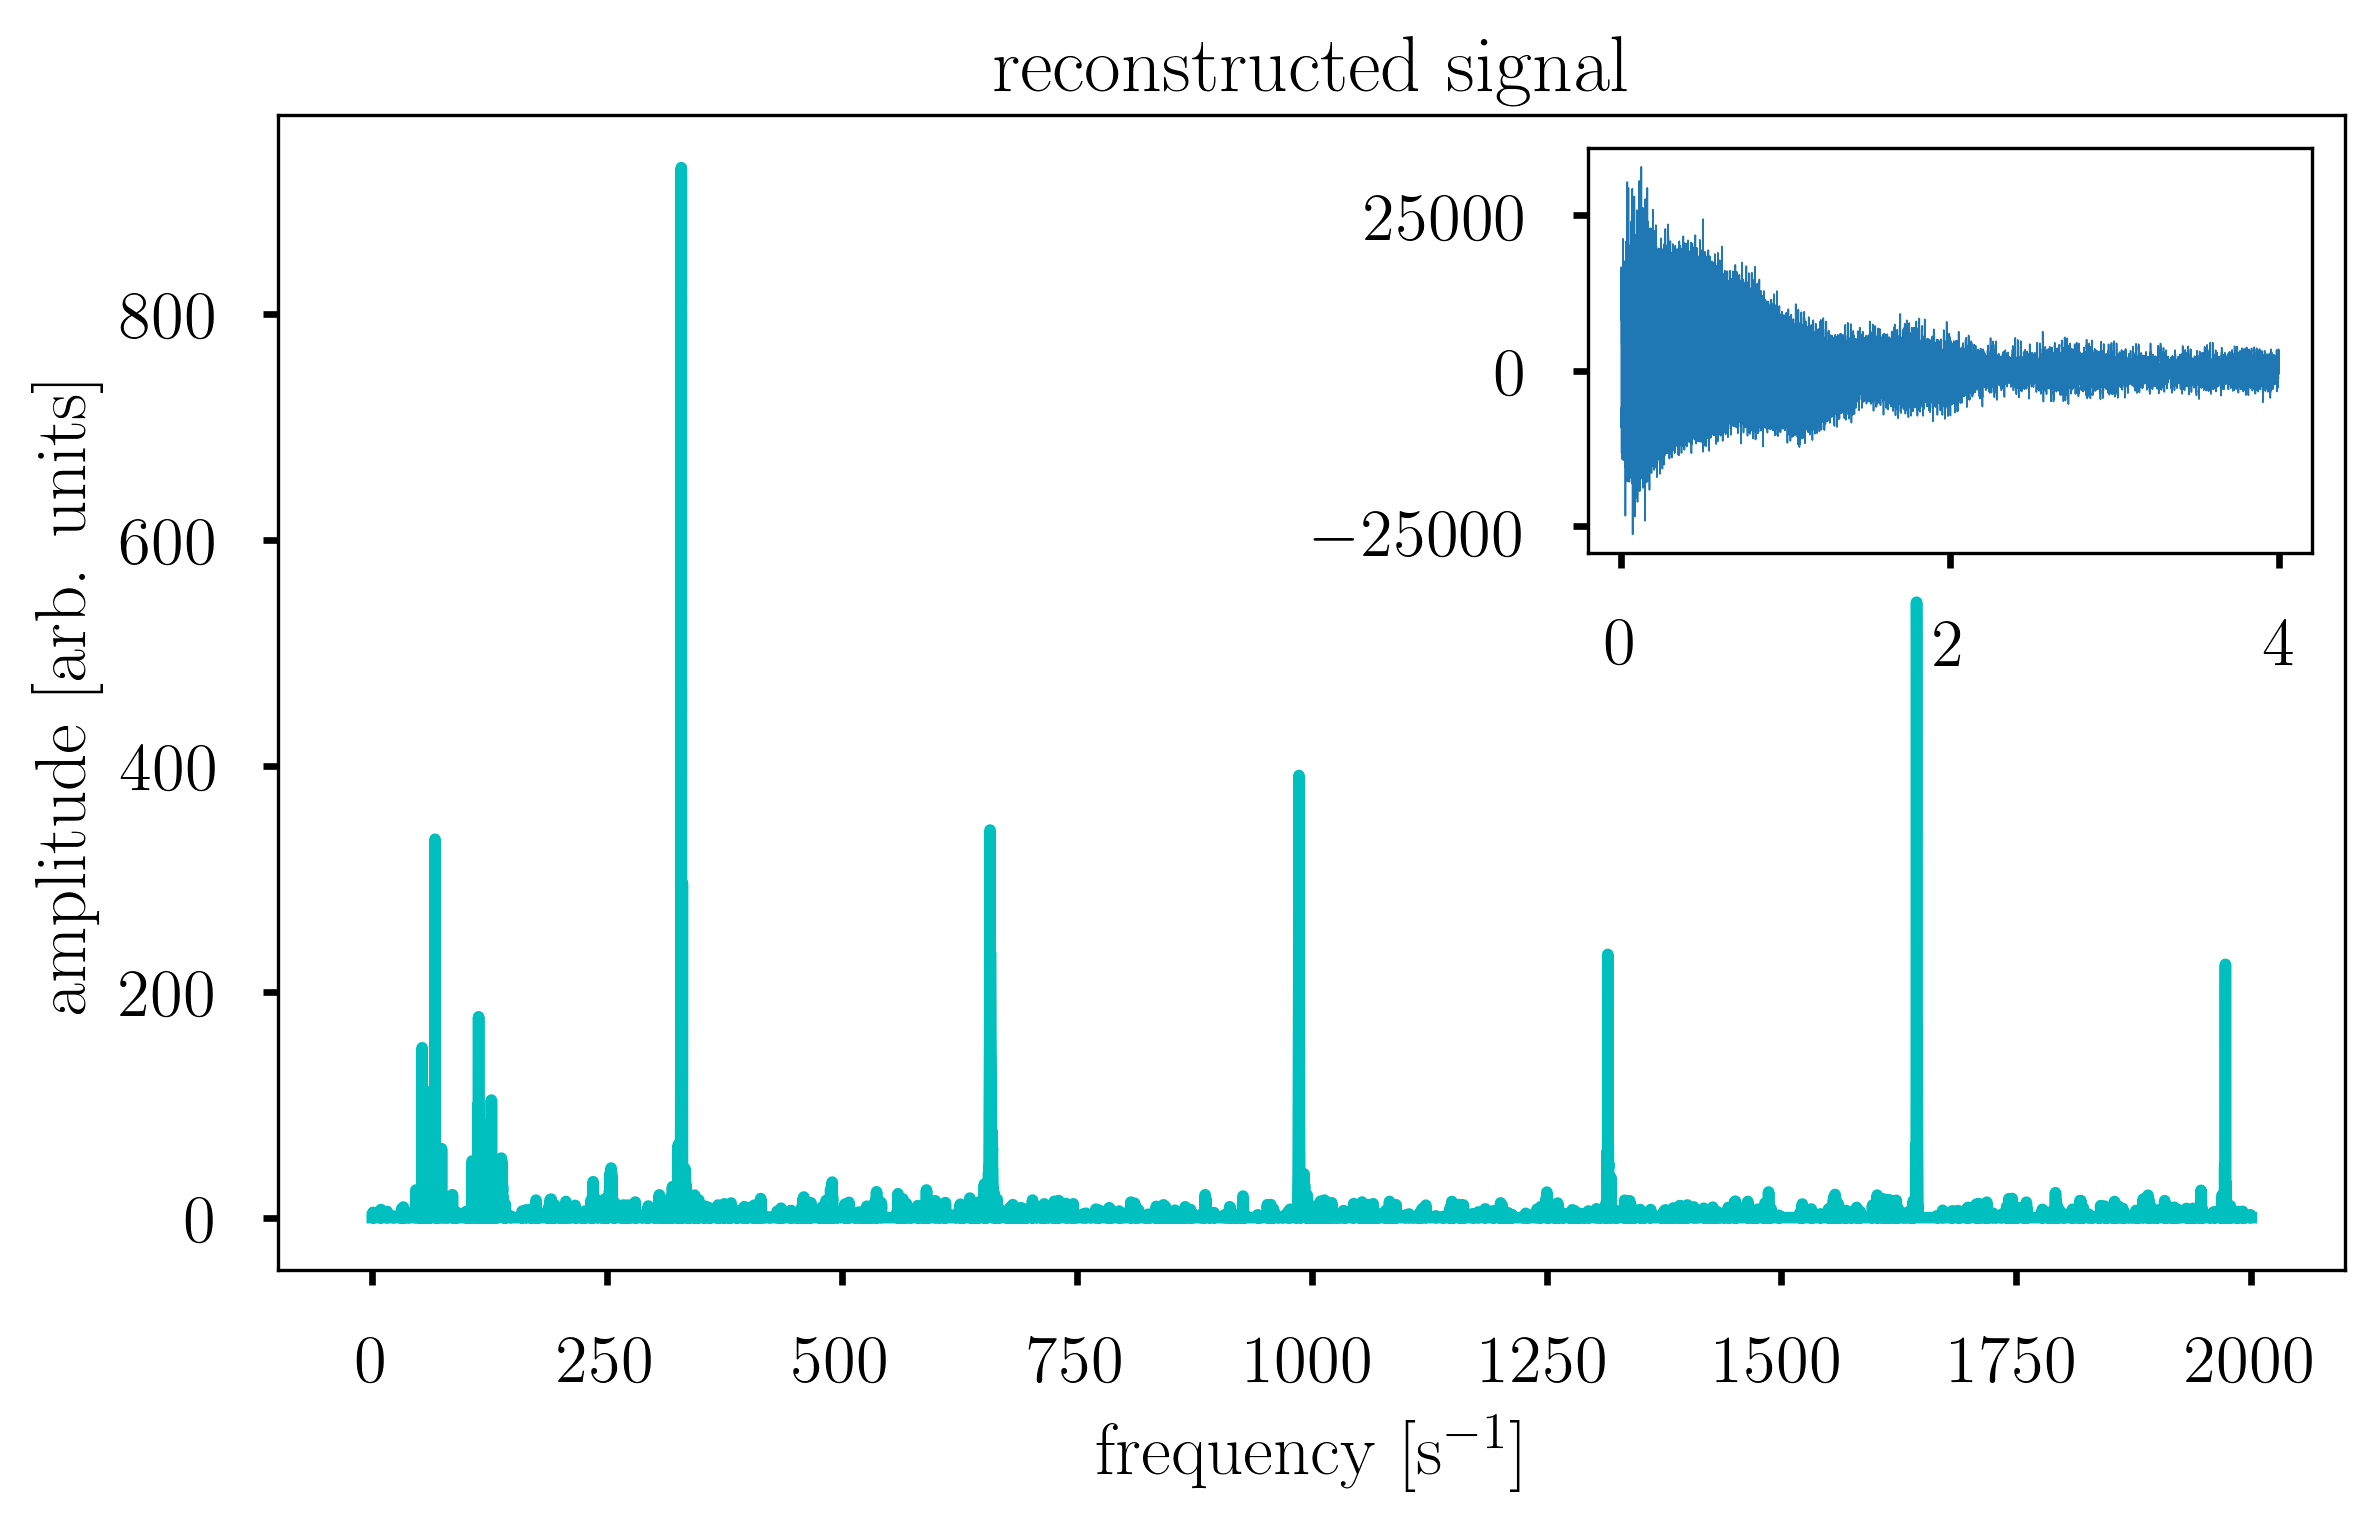
\includegraphics[width=\linewidth]{E1_recon_lasso.png}
		\caption{reconstructed signal}
		\label{fig:record-recon-lasso}
	\end{subfigure}
	\caption{Temporal and frequency domain representations of the guitar signal at 330 Hz.}
\end{figure}

\begin{figure}[!htb]
	\centering
	\begin{subfigure}{0.43\linewidth}
		\centering
		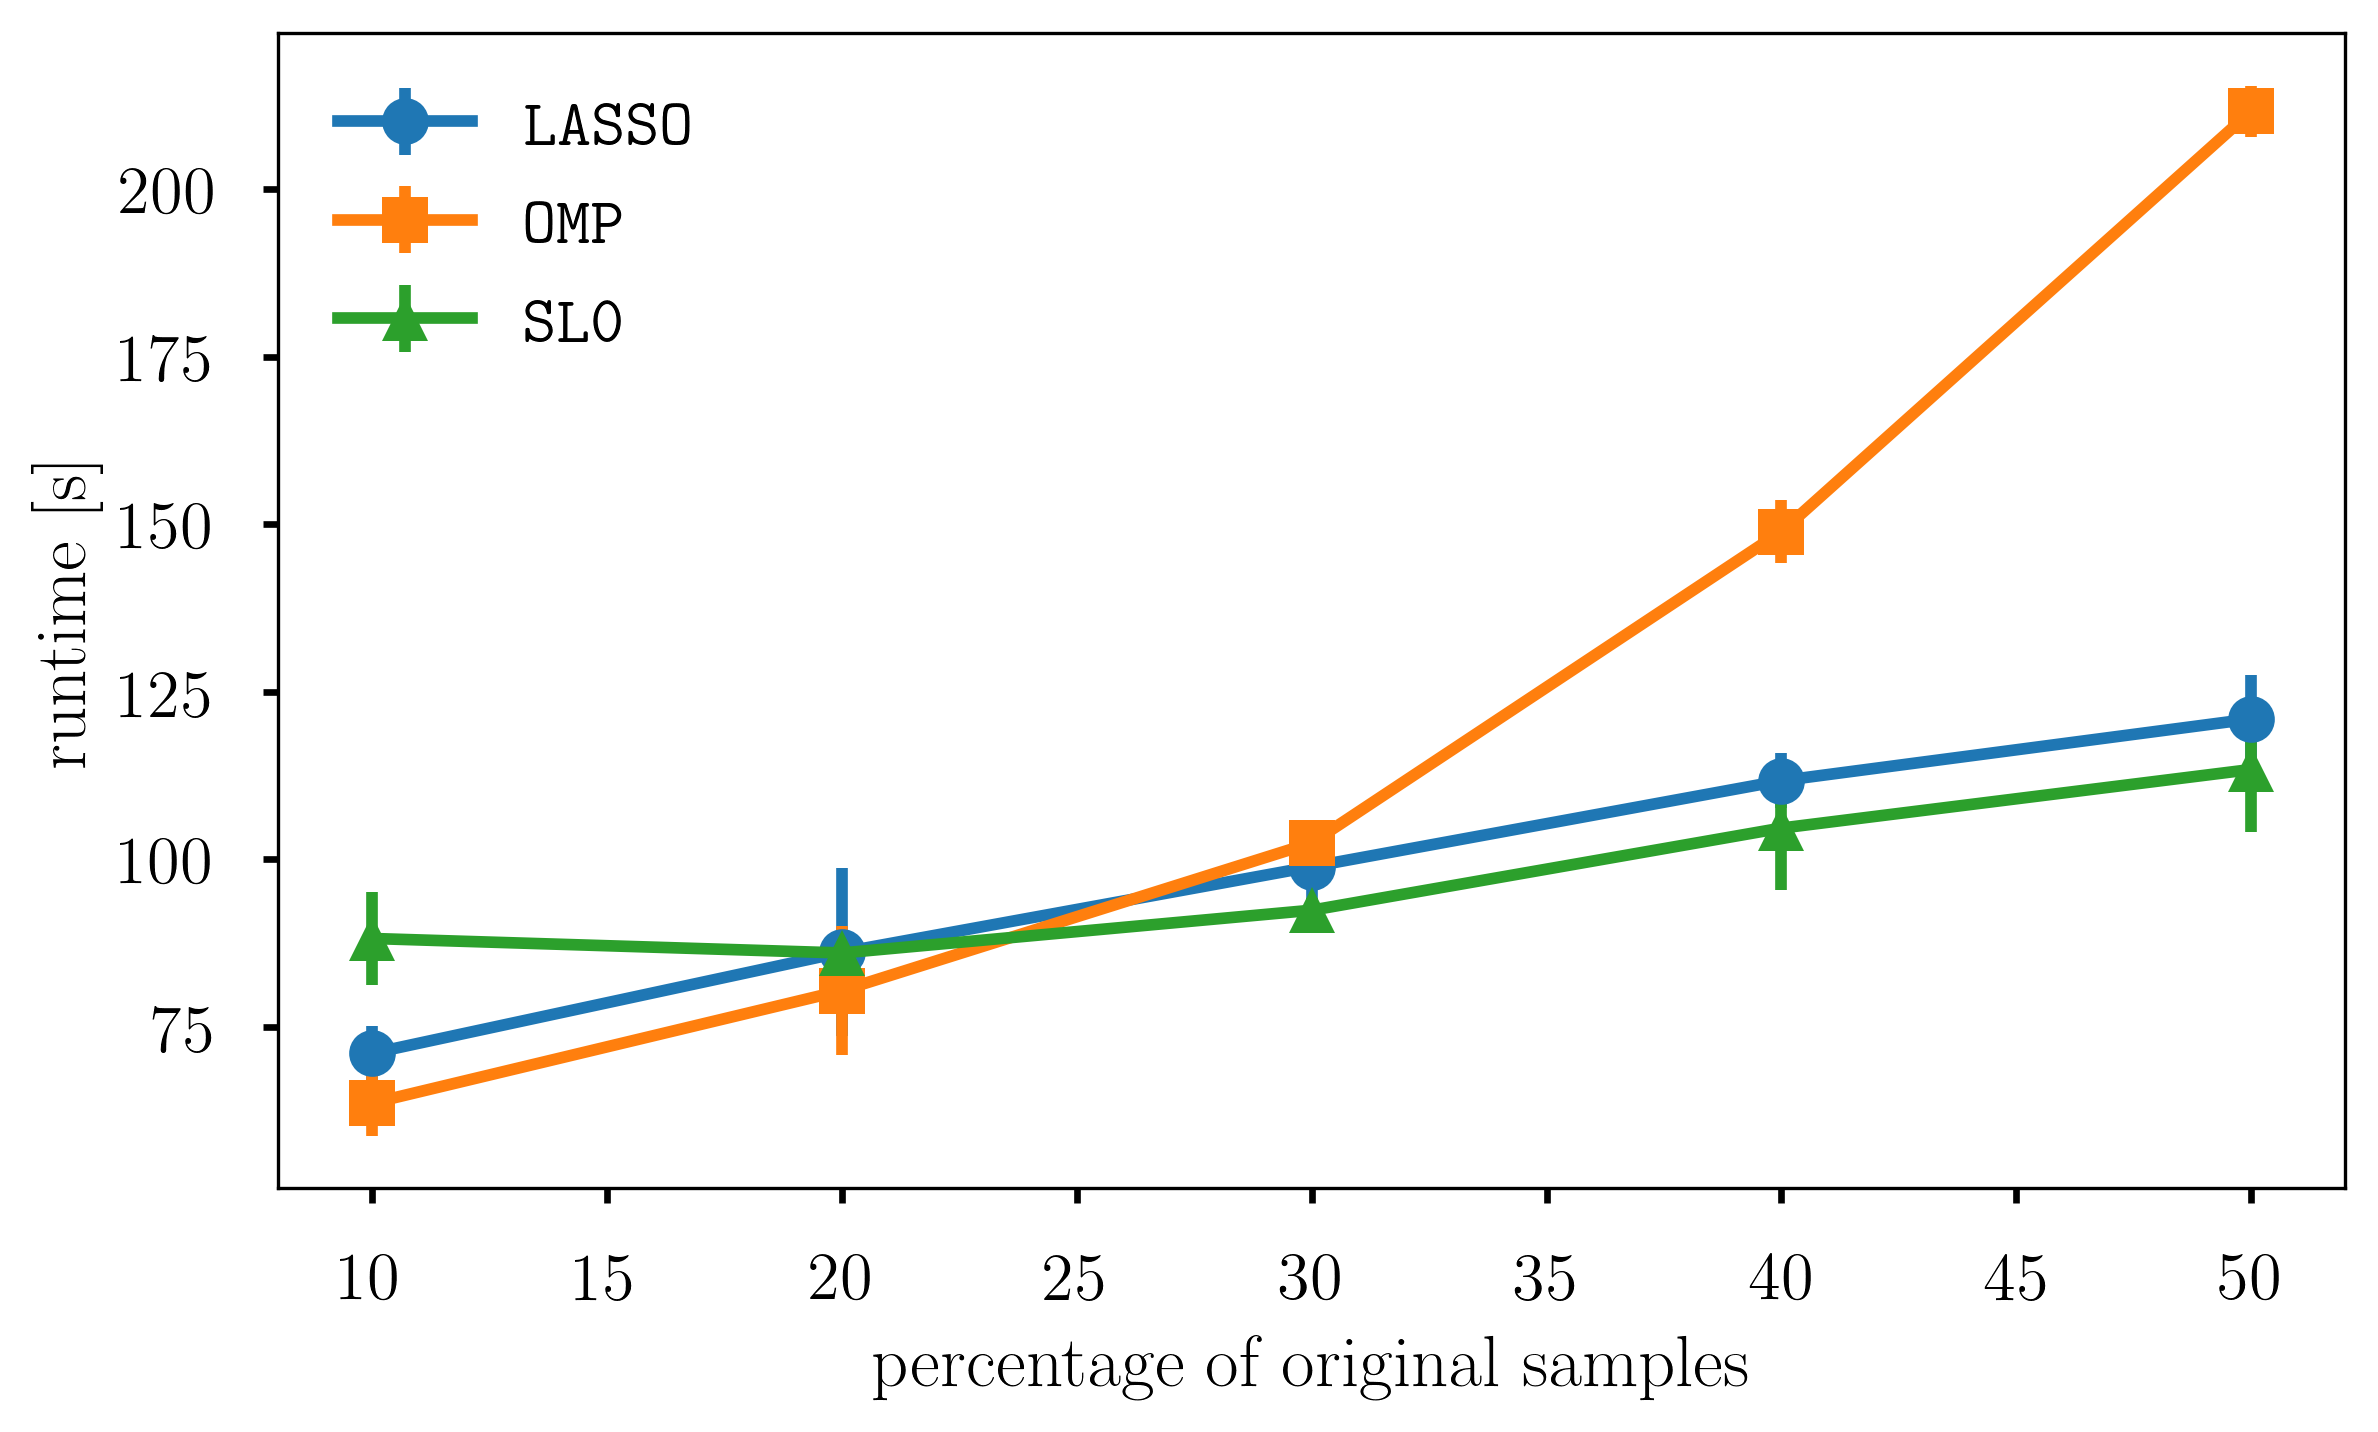
\includegraphics[width=\linewidth]{processtime.png}
		\caption{Computation time}
		\label{fig:process-time}
	\end{subfigure}
	\begin{subfigure}{0.43\linewidth}
		\centering
		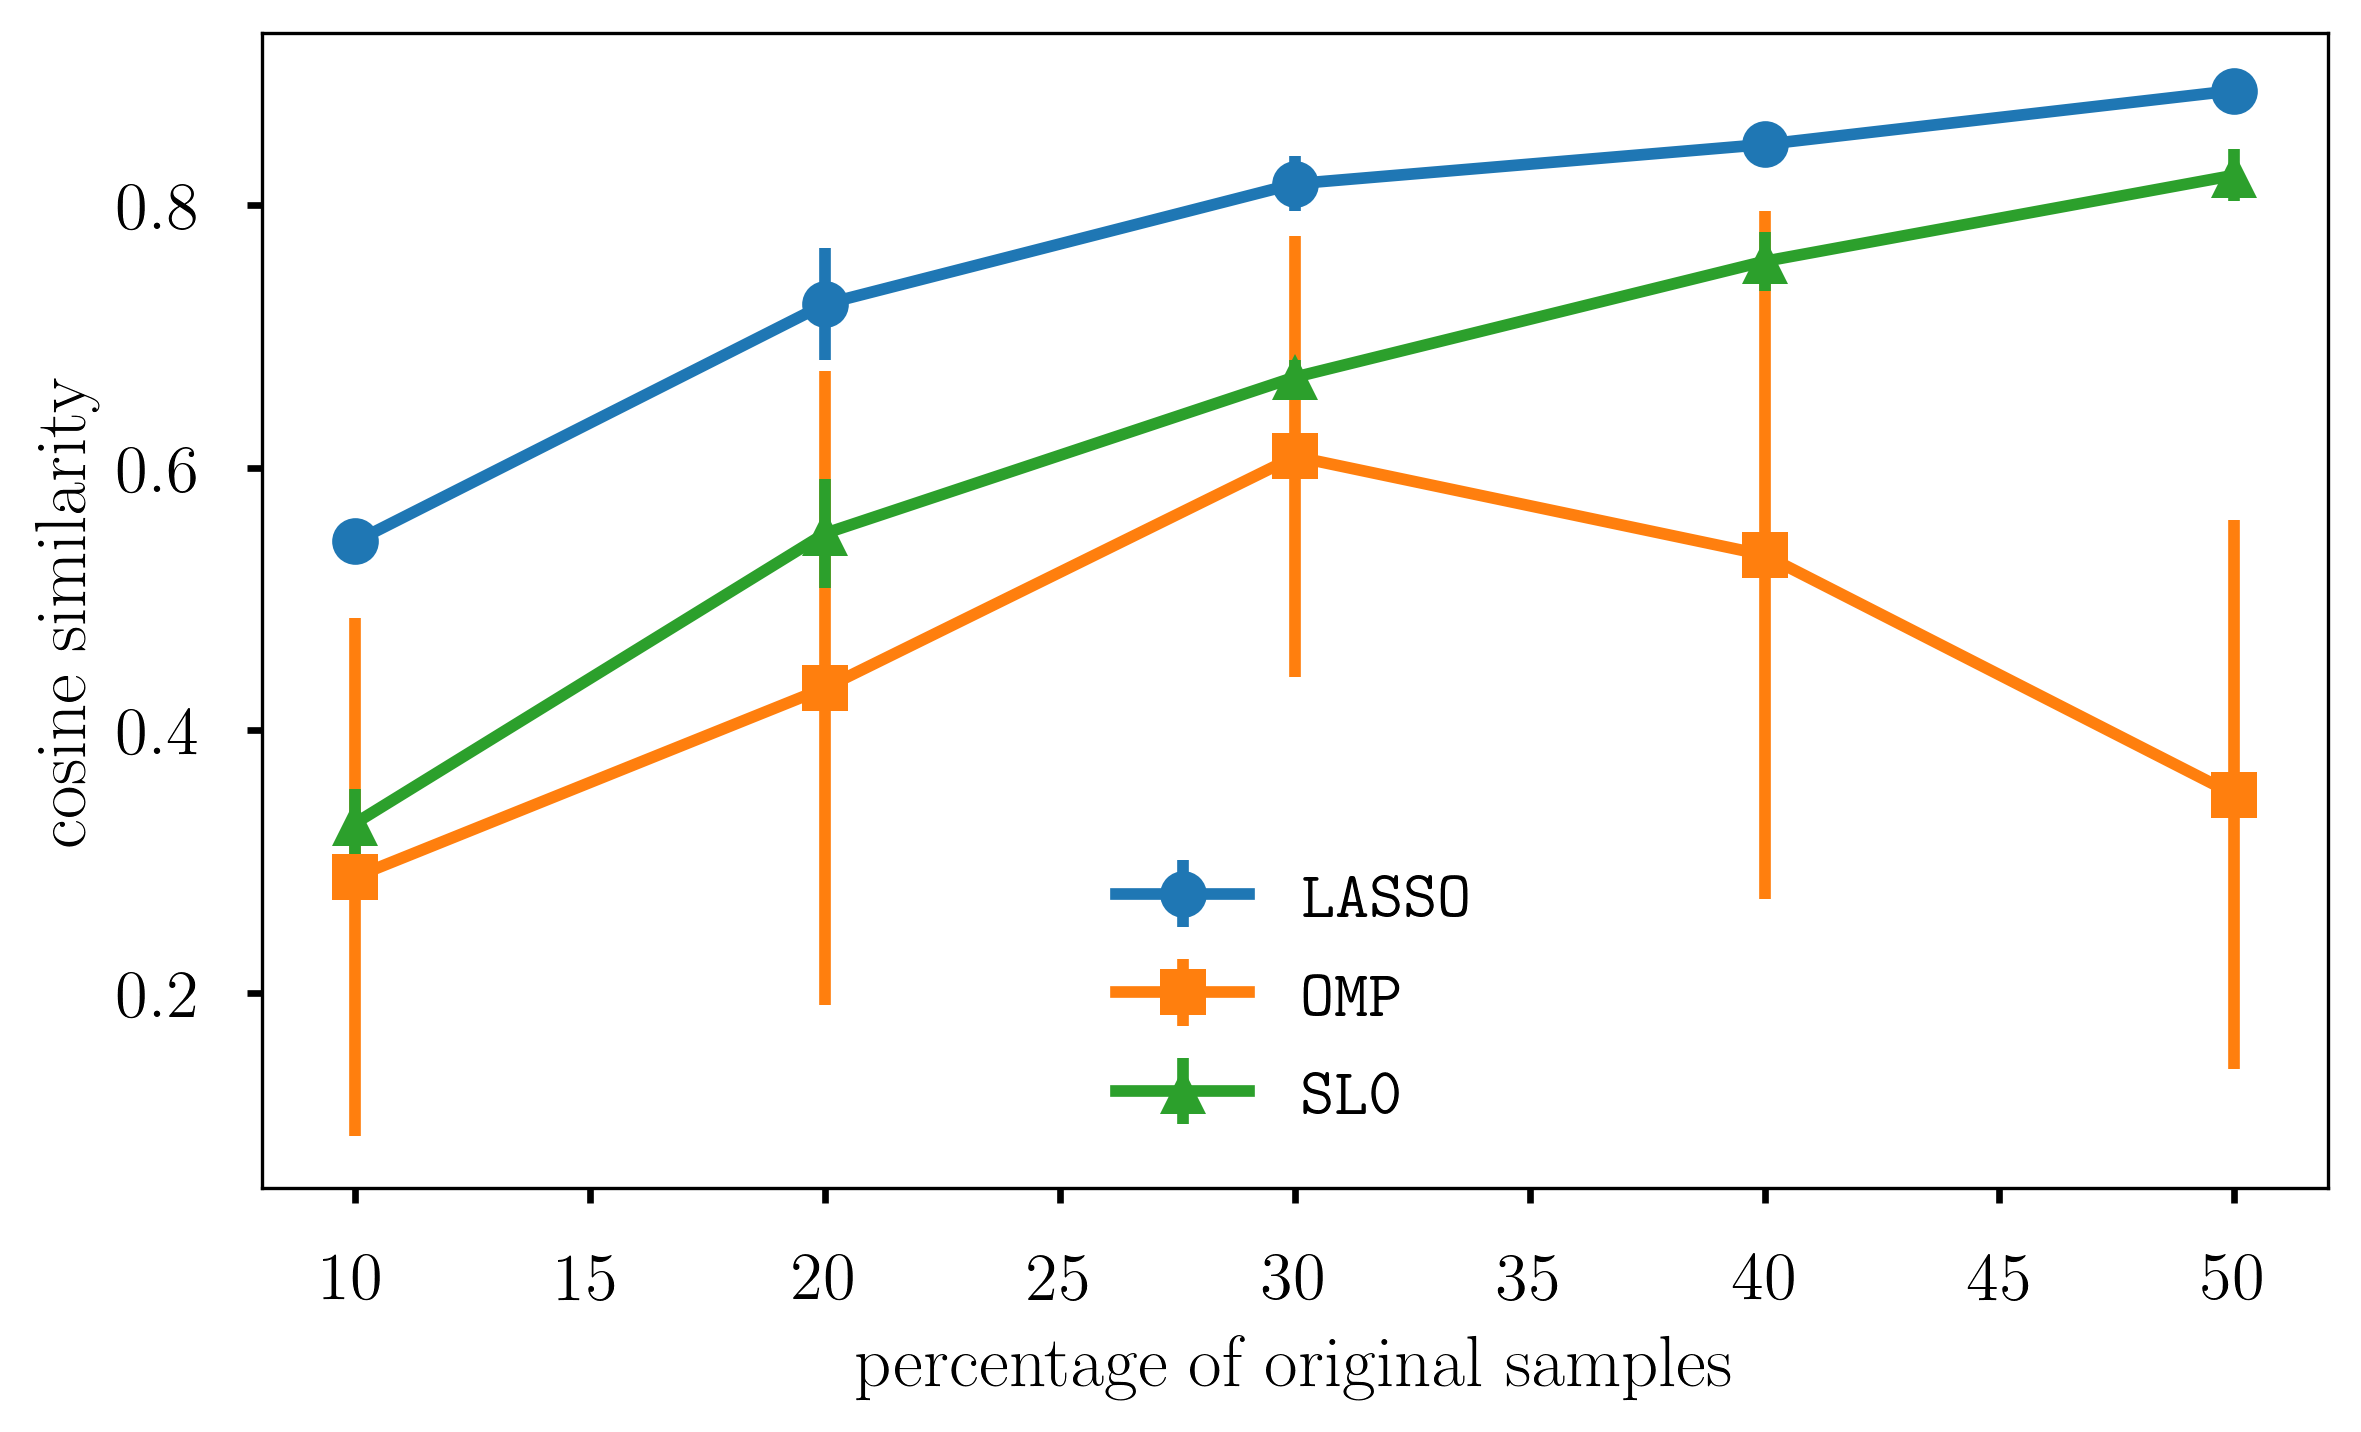
\includegraphics[width=\linewidth]{cossim.png}
		\caption{Cosine similarity}
		\label{fig:cossim}
	\end{subfigure}
	\caption{Comparison of performances of three algorithms for 10--50\% of samples, average over 10 iterations.}
	\label{fig:comparison}
\end{figure}


\section{Conclusions}\label{sec:Conc}
Audio was shown to have good reconstruction potential when stochastically sampled at a rate much lower than that required by the NSST. The recovery of higher-order harmonics was also demonstrated while being able to distinguish it from noise or erroneously reconstructed non-zero coefficients, even when sampling at a rate below that harmonic's frequency. The CS algorithm was applied on a recorded guitar playing a single note, and the quality of reconstruction was shown in the temporal and frequency representations of the signal. Comparison of the three different reconstruction algorithms used, namely LASSO, OMP, and SL0, showed that although runtimes vary, LASSO is superior in terms of reconstruction accuracy.

%\section*{Acknowledgments}


% Please use the style file spp-bst.bst. If you wish to use BibTeX, kindly use us the filename bibfile.bib 
%for your bib file.

\bibliographystyle{spp-bst}
\bibliography{compbib}

\end{document}